\begin{figure}[!h]
  \vskip -0.25cm
  \begin{center}
    \ifshort
    %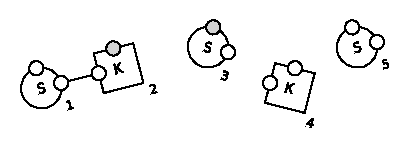
\includegraphics[scale=1.0]{figures/mixture-compact.pdf}
    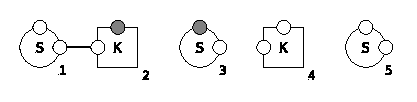
\includegraphics[scale=1.0]{figures/mixture-linear.pdf}
    \else
    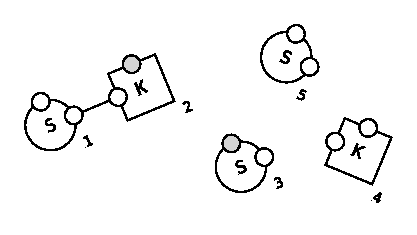
\includegraphics[scale=0.9]{figures/mixture.pdf}
    \fi
  \end{center}
  \vskip -0.5cm
  \caption{A mixture graph. Sites should be named, but are here simply
    identified through their position on agents\longversion{
      (phosphorylation sites are always shown on top). The relative
      position of agents in the figure is insignificant}.  Sites in a
    phosphorylated state are shown in gray. Number labels are global
    agent identifiers.}
  \label{fig:mixture}
\end{figure}